\section{Feature Matching}
\label{sec:methodology:featurematch}

The classification of biometrics speeds up the identification process by reducing the number of comparisons that must be made. There are two kinds of classification techniques: exclusive classification and continuous classification. Both fingerprint [14] and palmprint classifications [15] make use of exclusive classification. The main problem of this technique is that it uses only a small number of classes and the samples are unevenly distributed between them, with more than 90\% of the samples being in just two or three classes. A further problem with exclusive classification is that when classification is performed automatically, it is necessary to handle errors and rejected samples gracefully, which is a hard problem in practice. In contrast, for continuous classification, samples are not partitioned into disjoint classes but rather associated with numerical vectors which represent features of the samples. These feature vectors are created through a similarity-preserving transformation so that similar samples are mapped into close points in the multi-dimensional space [19]. In this paper, we adopt the continuous classification technique. As the global features combining MD, HCA and RLL are high-dimensional, we reduce the dimensions using the LDA method. We then improve the efficiency of palmprint recognition by applying coarse-level matching and Ranking Support Vector Machine (RSVM) to the low dimensional vectors.

\subsection{Dimension Reduction}
\label{ssec:methodology:lda}

LDA is a state-of-the-art dimensionality reduction technique widely used in classification problems. The objective is to find the optimal projection which simultaneously minimizes the within-class distance and maximizes the between-class distance, thus achieving maximum discrimination (Here, the “class” is used to denote the identity of the subjects, e.g. the samples collected from one palm are regarded as one class). However, the traditional LDA requires the within-class scatter matrix to be nonsingular, which means the sample size should be large enough compared with its dimension, but is not always possible. In this paper, we therefore adopt the orthogonal LDA (OLDA) proposed in [17], where the vectors of the optimal projection are calculated using the training database and the optimal projecting vectors are orthogonal to each other.
Suppose the 3D ROI has been divided to N levels and that M radial lines are used to represent the level contours. We can list the global features as a column vector,  , with   rows. Given a training database which has n samples and k classes as  , where   and  , adopting OLDA [17] the optimal projection W can be calculated as follows.
First, the within-class scatter matrix  , the between-class scatter matrix   and total scatter matrix   can be expressed as
                              (6)
where
                           (7)
                         (8)
                                         (9)
where   is the centroid of the ith class  ,   is the centroid of all the training samples ,   and  .
After calculating  ,   and  , the reduced Singular Value Decomposition (SVD) is applied to  .
                                     (10)
Denote   and compute the SVD of B.
                                          (11)
Let
                                              (12)
                                              (13)
and denote   the first   columns of the matrix D. Then, compute the QR decomposition of  .
                                    (14)
where Q is the desired orthogonal matrix and optimal projection, i.e.  .
After getting the optimal projection W, we can map the   dimensional vector F to a lower dimensional space
                                             (15)
where   is a   dimensional vector with  .

%!TEX root = featurematch.tex
\subsection{Coarse-level Matching}
\label{ssec:methodology:naive}

For palmprint recognition, we need a measurement of similarity between two samples. If the similarity is high, we have a high confidence to believe that the two samples are from the same person. Otherwise we reject to claim that.

After mapping the high-dimensional feature vector to $\Gamma$-dimensional vector $\tilde{F}$, the similarity between two samples can be calculated as

\begin{equation}
Similarity= \| \tilde{F}_1 -\tilde{F}_2 \|
= \sum \limits_{i=1}^{\Gamma} (f_i^1-f_i^2)^2
\label{eq:methodology:similarity}
\end{equation}

\begin{figure}[htb]
  \begin{center}
    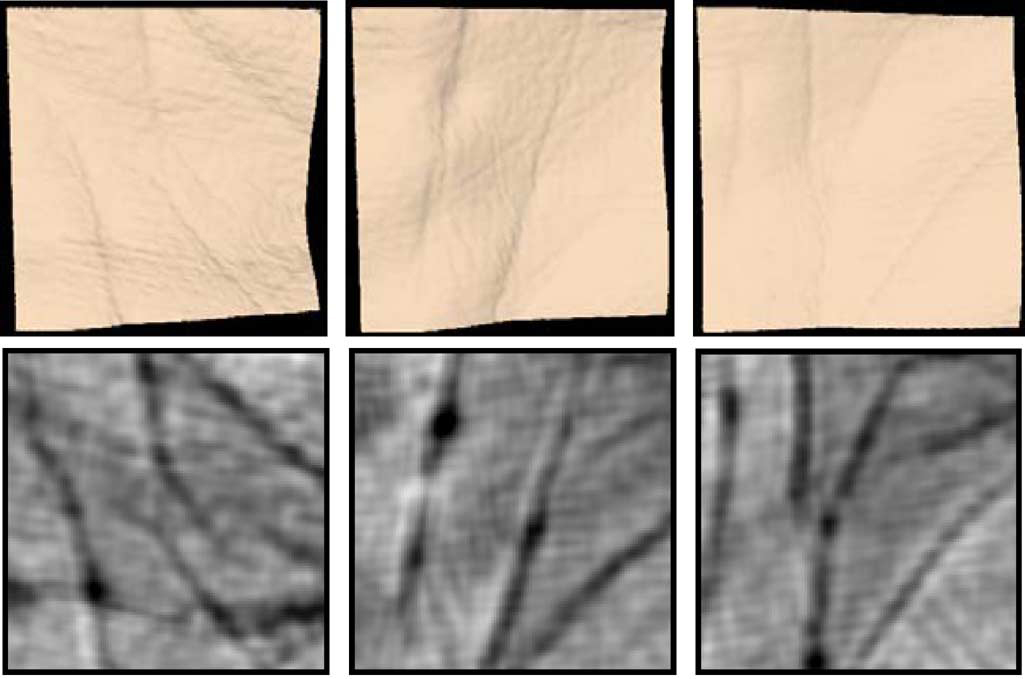
\includegraphics[width=0.9\linewidth]{ch-methodology/figures/mci1}
    \caption[MCI for ROIs from different palms]{Mean Curvature Image for ROIs from three different palms}    \label{fig:methodology:mci1}
  \end{center}
\end{figure}

\begin{figure}[htb]
  \begin{center}
    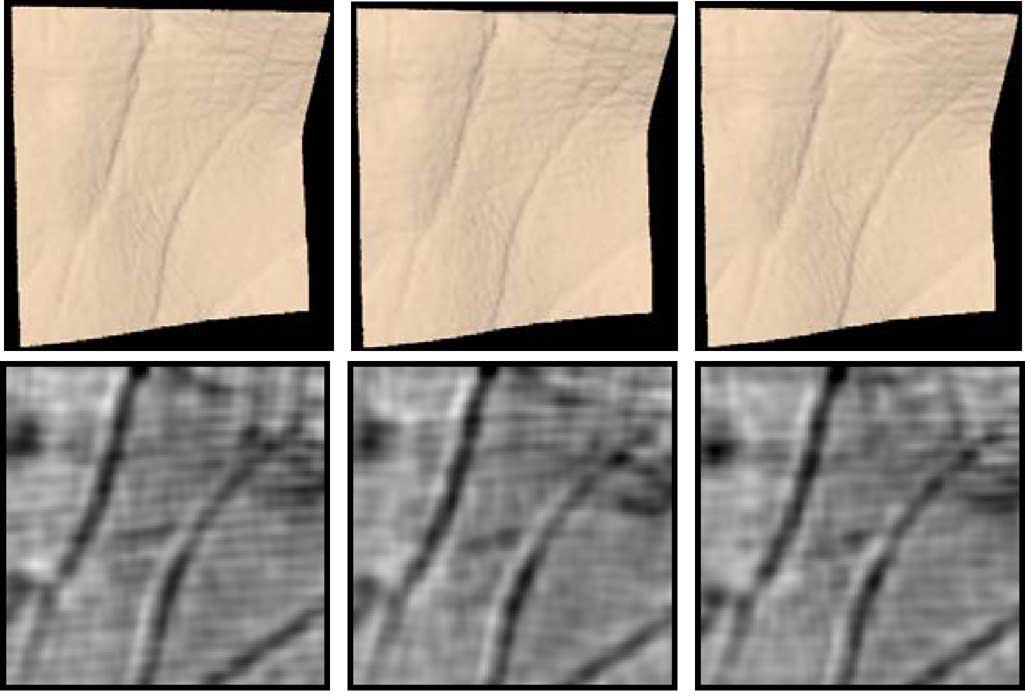
\includegraphics[width=0.9\linewidth]{ch-methodology/figures/mci2}
    \caption[MCI for ROIs from the same palm]{Mean Curvature Image for ROIs from three samples of the same palm}    \label{fig:methodology:mci2}
  \end{center}
\end{figure}

There are other features extracted from the same dataset such as Mean Curvature Image in ~\cite{Zhang:2009dp}. Figure ~\ref{fig:methodology:mci1} shows the ROI and MCI extracted from three different palms while Figure ~\ref{fig:methodology:mci2} show samples from the same palm. The corresponding matching score is defined as

\begin{equation}
Y=\frac{
    2\sum \limits_{i=1}^{n} \sum \limits_{j=1}^{m} Z_d(i,j) \cap Z_t(i,j)
}
{
    \sum \limits_{i=1}^{n} \sum \limits_{j=1}^{m} Z_d(i,j) +
    \sum \limits_{i=1}^{n} \sum \limits_{j=1}^{m} Z_t(i,j)
}
\end{equation}

where symbol $\cap$ represents the logical AND operation, $Z_d$ and $Z_t$ are two binarized MCIs. Due to the fact that MCI is covariant to shifting, the actual matching process for MCI is repeated by shifting the image with 4 different displacement in 8 directions. A total of 33 matching scores are calculated and the maximum is adopted as the overall matching score.

Although MCI feature is more descriptive, it takes up more storage ($200\times200$ floats to store the feature image). Compared to the computation in ~\ref{eq:methodology:similarity}, the MCI matching process requires far more computation and is therefore significantly slower.
% Table generated by Excel2LaTeX from sheet 'Sheet1'
\begin{table}[htbp]
  \centering
  \caption{Penetration rate and error rate using RSVM}
    \begin{tabular}{|c|c|}
    \hline
    Penetration rate (\%) & Error rate (\%) \\
    \hline
    30    & 1.3 \\ \hline
    27.5  & 1.33 \\ \hline
    25    & 1.37 \\ \hline
    22.5  & 1.42 \\ \hline
    20    & 1.49 \\ \hline
    17.5  & 1.63 \\ \hline
    15    & 1.87 \\ \hline
    12.5  & 2.48 \\ \hline
    10    & 3.35 \\ \hline
    7.5   & 4.41 \\ \hline
    5     & 5.88 \\
    \hline
    \end{tabular}%
  \label{tab:experiment:svm}%
\end{table}%
